\documentclass{article}
\usepackage[cm]{fullpage}
\usepackage{indentfirst}
%----------figure layout style
\usepackage{float}
\usepackage{graphicx}
\usepackage{subfigure}
\usepackage[small,bf]{caption}

\title{a brief comparison of control schemes on exoskeleton}
%\author{Suresh Kumar Gadi}
\author{}

\begin{document}
\maketitle
\section{Introduction}
In this report we show a generalized scheme to understand the interaction between exoskeleton and human body. Later part of this report shows how different control schemes fit in the given scheme. This report allows us to observe the differences in the control schemes. Stability proof or performance for the different control schemes are not studied in this report.
\section{A generalised approach to study exoskeleton}
\begin{figure}
  \centering
  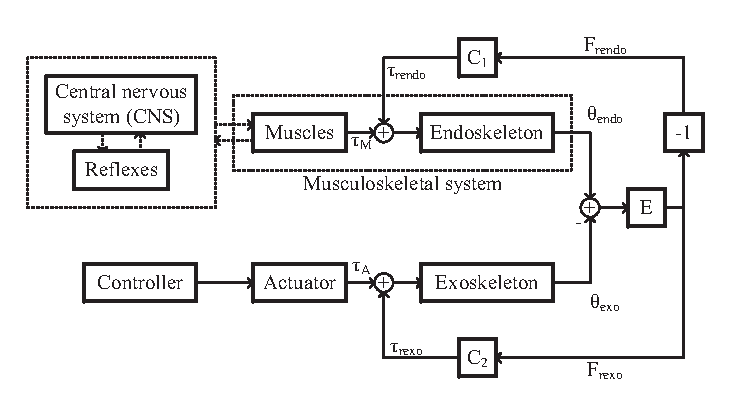
\includegraphics[width=09cm]{images/General_BD.eps}\\
  \caption{Generalised block diagram showing endoskeleton and exoskeleton}\label{Fig:General_BD}
\end{figure}
Figure \ref{Fig:General_BD} shows a possible interaction between a human arm and an exoskeleton arm. Servo hypothesis suggests that a desired path for a human arm is generated in the Central nervous system (CNS),  which is passed to a muscle through the spinal chord. The spinal chord receives a feedback from the muscles, which allows the spinal chord to control the movement of a arm. An actuator controlled by a computer powers the exoskeleton arm. The difference in human arm position ($\theta_{endo}$) and exoskeleton arm position ($\theta_{exo}$) causes a force, which can be written as
\begin{eqnarray}
    F_{rexo} = - F_{rendo} = E(\theta_{endo}-\theta_{exo}) \label{Eqn:Reaction_Force}
\end{eqnarray}
where $E(.)$ is a nonlinear function which maps difference in $\theta_{endo}$ and $\theta_{exo}$ to a reaction force generated on exoskeleton arm ($F_{rexo}$) and human arm ($F_{rendo}$). The reaction torque experienced by human arm ($\tau_{rendo}$) and exoskeleton arm ($\tau_{rexo}$) can be given as
\begin{eqnarray}
    \tau_{rendo} &=& C_1F_{rendo} \label{Eqn:taurendo} \\
    \tau_{rexo} &=& C_2F_{rexo} \label{Eqn:taurexo}
\end{eqnarray}
where $C_1$ and $C_2$ are positive constants.
\par
In the following sections, we will discuss different control schemes applied to achieve exoskeleton arm to follow a human arm trajectory.
\section{Kazerooni's algorithm (1988) \cite{SGadi:Kazerooni88}}
\begin{figure}
  \centering
  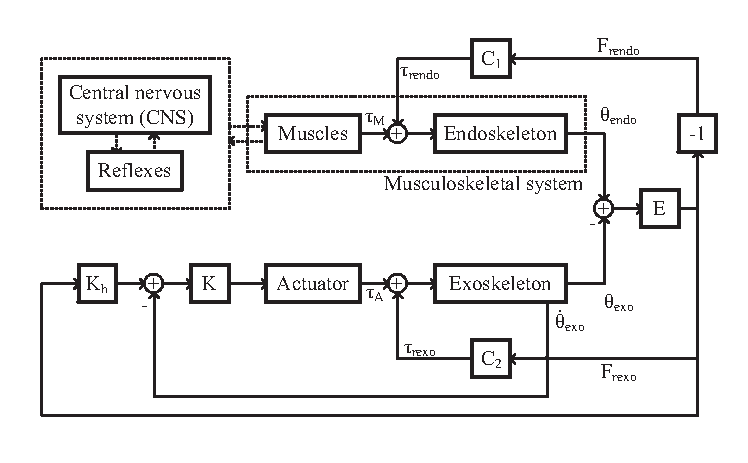
\includegraphics[width=09cm]{images/Kazerooni_BD.eps}\\
  \caption{Control scheme equivalent to the control scheme proposed in \cite{SGadi:Kazerooni88}}\label{Fig:Kazerooni_BD}
\end{figure}
The dynamics of CNS, endoskeleton, and $E(.)$ are approximated to a linear dynamic model for simplicity. This control scheme is shown in Figure \ref{Fig:Kazerooni_BD}. $K_h$ and $K$ are linear dynamic systems. In this control scheme, the exoskeleton arm velocity is controlled. The difference in the human arm position and the exoskeleton arm position causes a velocity in the exoskeleton arm towards to cancel this difference in position. $F_{rexo}$ is measured using force sensor. We can notice that the exoskeleton arm position stays stationary in case user is having no interaction with the force sensor.
\section{BLEEX algorithm (2005) \cite{kazerooni2005control}}
\begin{figure}
  \centering
  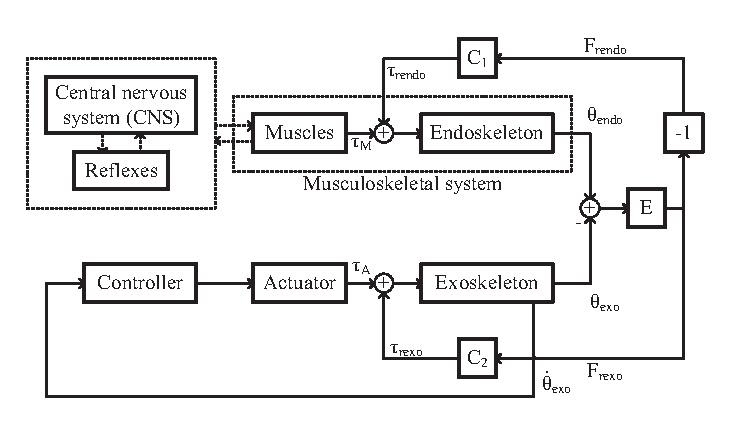
\includegraphics[width=09cm]{images/BLEEX_BD.eps}\\
  \caption{Control scheme equivalent to the control scheme proposed in \cite{kazerooni2005control}}\label{Fig:BLEEX_BD}
\end{figure}
This control scheme does not use any force sensor. In this control scheme, a positive feed back loop is used to increase the sensitivity to the external disturbances. Figure \ref{Fig:BLEEX_BD} shows this control scheme, where the $\tau_{rexo}$ generates the external disturbances. Due to high sensitivity towards external disturbances, the exoskeleton arm follows the human arm. The controller used in this control scheme needs to implement accurately inverse dynamics of exoskeleton arm and actuator, which needs a accurate model of actuator and exoskeleton arm.
\section{Tomizuka's algorithm (2009) \cite{kong2009control}}
\begin{figure}
  \centering
  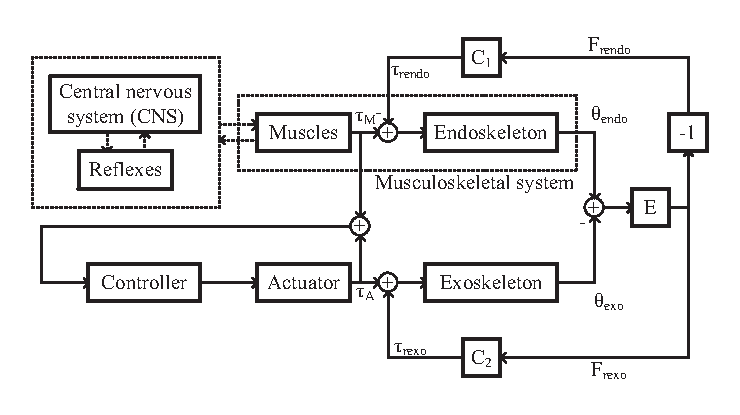
\includegraphics[width=09cm]{images/Tomizuka_BD.eps}\\
  \caption{Control scheme equivalent to the control scheme proposed in \cite{kong2009control}}\label{Fig:Tomizuka_BD}
\end{figure}
This control scheme needs a positive feedback of the sum of the torques exerted by the muscles and the actuator. The actuator dynamics are neglected by introducing a proper cancelation to these dynamics into the controller. The torque exerted by the muscles can be estimated by a EMG sensor, a muscle hardness sensor, or a muscle fiber expansion sensor. Since this control scheme uses a positive feedback, the closed-loop sensitivity for the torque exerted by the muscles is high.
\section{Gadi's algorithm (2016) \cite{gadi2016stability}}
\begin{figure}
  \centering
  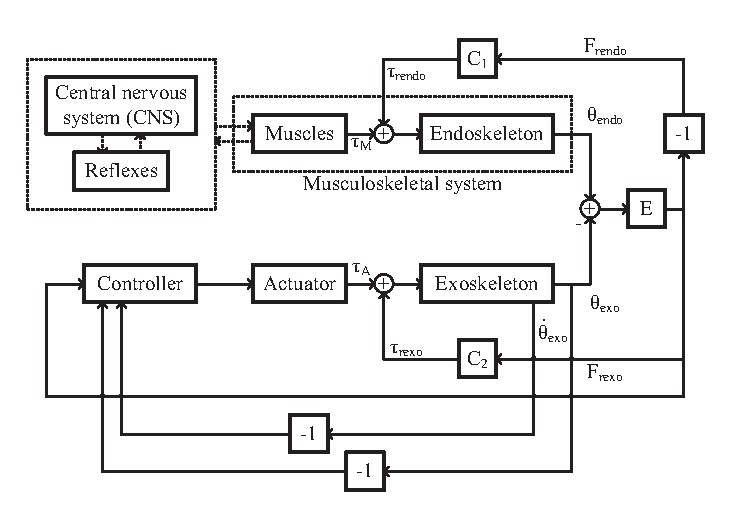
\includegraphics[width=09cm]{images/Our_BD.eps}\\
  \caption{Our control scheme}\label{Fig:Our_BD}
\end{figure}
In our control scheme, we are using a linear model for CNS, spinal chord, muscles and endoskeleton human arm. We are using an approximation of $E(.)$ as a constant. The actuator dynamics are neglected by introducing inverse dynamics of actuator in the controller. The controller provides an amplifying effect of $\tau_{rexo}$. We can notice that the actuator does not provide any torque while human arm is released, which will bring the exoskeleton to the equilibrium point. Additionally controller provides a velocity and position feedback for obtaining desired performance under no human contact.
\bibliographystyle{unsrt}
\bibliography{../refs}
\end{document}

